\documentclass[simplex.tex]{subfiles}
% NO NEED TO INPUT PREAMBLES HERE
% packages are inherited; you can compile this on its own

\onlyinsubfile{
\title{NeuroData SIMPLEX Report: Subfile}
}

\begin{document}
\onlyinsubfile{
\maketitle
\thispagestyle{empty}

The following report documents the progress made by the labs of Randal~Burns and Joshua~T.~Vogelstein at Johns Hopkins University towards goals set by the DARPA SIMPLEX grant.

%%%% Table of Contents
\tableofcontents

%%%% Publications
\bibliographystyle{IEEEtran}
\begin{spacing}{0.5}
\section*{Publications, Presentations, and Talks}
%\vspace{-20pt}
\nocite{*}
{\footnotesize	\bibliography{simplex}}
\end{spacing}
%%%% End Publications
}


\subsection{FlashX}

Sparse matrix multiplication in FlashX uses its own format (SCSR) for sparse
matrices to improve computation efficiency. We investigated the overhead of
using customized format to thoroughly evaluate the computation efficiency of
sparse matrix multiplication in FlashX. Thus, it is essential to accelerate the
format conversion from a standard format such as CSR to our customized
format SCSR. Figure \ref{fig:flashx1}, below, shows the benefit of using
the SCSR format including the overhead of format conversion. When an
application requires more than 4 SpMVs, converting the format of a
sparse matrix improves the computation efficiency of the application. Thus,
majority of the applications benefit from the format conversion.

\begin{figure}[h!]
\begin{cframed}
\centering
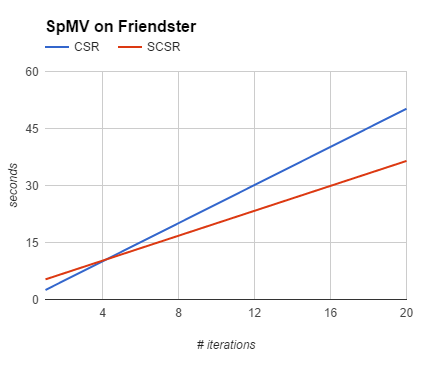
\includegraphics[width=0.45\textwidth]{../../figs/SpMV-friendster.png}
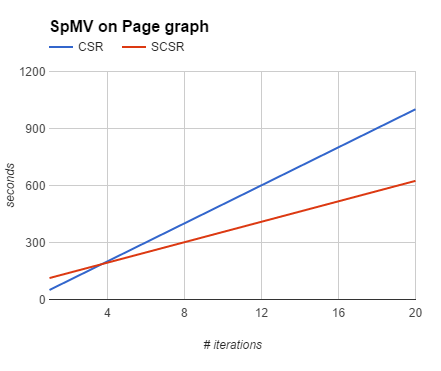
\includegraphics[width=0.45\textwidth]{../../figs/SpMV-pagegraph.png}
\caption{
Benefits of using SCSR on real-world datasets. The Friendster graph has
65 million vertices and
1.8 billion edges. The page graph has 3.4 billion vertices and 129 billion
edges. Although there is some overhead in converting data to SCSR format,
after only 4 iterations, this overhead is more than offset by the increase
speed per iteration. In typical applications, we use $\sim 20$ iterations.
}
\label{fig:flashx1}
\end{cframed}
\end{figure}

%The speed ratio of the in-memory and semi-external memory sparse
%matrix multiplication in FlashX is affected by multiple factors. Shown
%in Figure \ref{fig:flashx2}, we demonstrate some of the factors with SBM
%graphs with the same number of vertices and edges. We vary the number of
%clusters and the number of edges inside clusters. We measure the computation
%efficiency of SpMV on both clustered and un-clustered graphs. When
%vertices are ordered based on the cluster structure, more clusters and
%more edges inside clusters increase CPU cache hits, which leads to less
%computation overhead and larger speed gap between in-memory and
%semi-external memory executions. However, if vertices are ordered
%randomly, these two factors have less obvious impact on speed.

%\begin{figure}[h!]
%\begin{cframed}
%\centering
%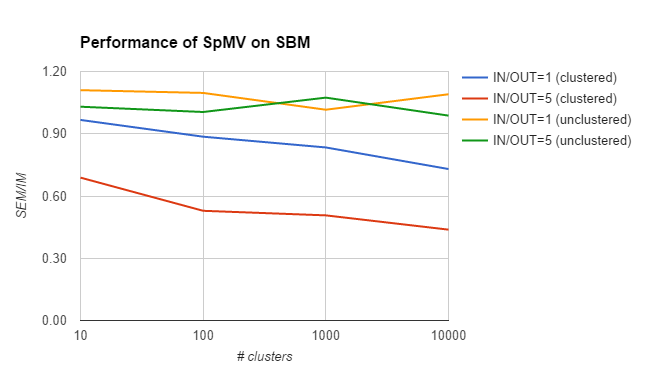
\includegraphics[width=0.75\textwidth]{../../figs/SpMV-sbm.png}
%\caption{
%The relative speed of our SpMV implementation on synthetic graphs
%generated from stochastic block model (SBM). The SBM graphs have 100 million
%vertices and 3 billion edges. IN/OUT indicates the ratio of edges inside
%and outside clusters. The vertices in a graph are ordered based on the cluster
%structures (clustered) or randomly ordered (unclustered). The speed of
%SpMV is affected by the structure of a graph. For example, the vertex ordering
%of a graph has significant impact in speed.
%}
%\label{fig:flashx2}
%\end{cframed}
%\end{figure}

We implement Daniel Lee's NMF algorithm with our semi-external memory
sparse matrix multiplication (denoted as SEM-NMF) and evaluate its
speed by comparing it with a high-performance NMF implementation
SmallK on billion-scale graphs. The dense matrices for NMF can be as
large as the sparse matrix. As such, we split the dense matrix
vertically so that each of the vertical partitions can fit in memory. We
also evaluate the effect of the memory size on the speed of
SEM-NMF by varying the number of columns in memory from the dense
matrices. In the experiment, we factorize each of the graphs
into two $n \times 16$ non-negative dense matrices.


We significantly improve the speed of SEM-NMF by keeping more
columns of the input dense matrix in memory (Figure \ref{fig:nmf}). The
speed improvement is more significant when the number of columns
that fit in memory is small. When we keep eight columns of the input
dense matrix in memory, SEM-NMF achieves over 60\% of the speed of
its in-memory execution.


SEM-NMF significantly outperforms SmallK and other NMF implementations
in the literature. SmallK is the closest competitor. We run the same NMF
algorithm in SmallK and SEM-NMF outperforms SmallK by a large factor on
all graphs (Figure~\ref{fig:nmf}). There are many MapReduce
implementations in the literature. They run on sparse matrices with tens
of millions of non-zero entries but generally take one or two orders of
magnitude more time than our SEM-NMF on the sparse matrices with
billions of non-zero entries.


\begin{figure}[h!]
\begin{cframed}
\centering
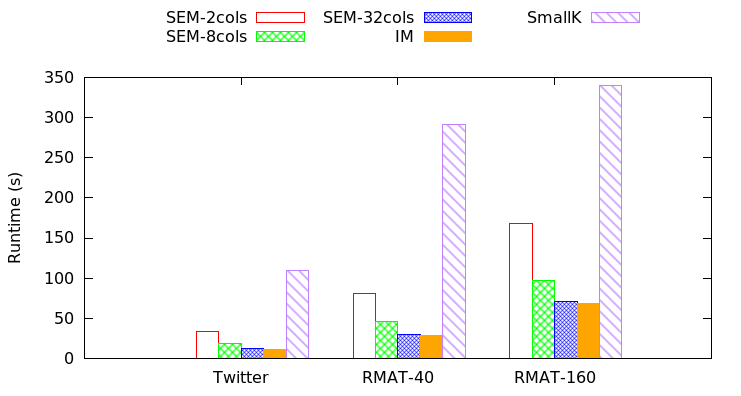
\includegraphics[width=0.5\textwidth]{../../figs/nmf.png}
\caption{
Performance of SEM-NMF on large directed graphs. The Twitter graph has
42 million vertices and 1.5 billion edges; RMAT-40 has 100 million vertices
and 3.7 billion edges; RMAT-160 has 100 million vertices and 14 billion
edges. SEM-NMF outperforms SmallK by a large factor for all different settings.
While using more memory to store columns in the dense matrices, SEM-NMF
gets higher speed.
}
\label{fig:nmf}
\end{cframed}
\end{figure}

\begin{figure}[h!]
\begin{cframed}
\centering
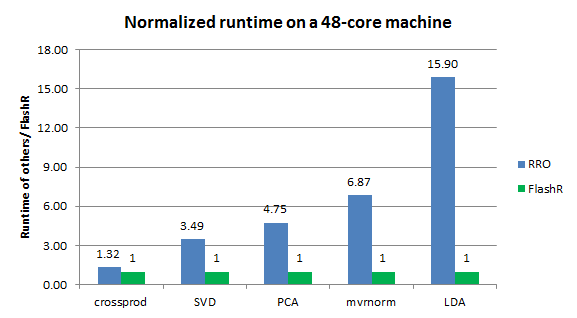
\includegraphics[width=0.5\textwidth]{../../figs/FlashR.vs.RRO.png}
\caption{
Normalized runtime of FlashR vs. Revolution R on a dataset with one million
data points and 1000 features when running R implementations of machine
learning primitives on a large parallel machine with
48 CPU cores. FlashR outperforms Revolution R in all operations. When
the computation gets more complex, the performance advantage of FlashR
over Revolution R gets larger.
}
\label{fig:flashr}
\end{cframed}
\end{figure}

In the past months, we significantly advanced FlashR in both compatibility with R
and efficiency. FlashR now overrides about 70 R matrix functions in the R
\textit{base} package. As such, we can run existing R code with little
modification or no modification at all. For example, we ported a few R
implementations of machine learning algorithms in the \textit{MASS} package
with little modification. We compare the speed of FlashR against Revolution R,
which is also designed to parallelize and accelerate R code, on a large parallel
machine with 48 CPU cores (Figure \ref{fig:flashr}).
Even for the simple matrix operation such as \textit{crossprod}, FlashR
outperforms Revolution R. As the computation gets more complex, the advantage
of FlashR over Revolution R gets larger. When executing the LDA implementation
(Linear Discriminant Analysis) in the MASS package, FlashR outperforms Revolution R
by an order of magnitude.


\end{document}
